% !Mode:: "TeX:UTF-8"

\chapter{使用聚类算法提高压缩率}

聚类算法是器学习中的一类经典算法,常用于数据分类与数据特征提取,聚类即物以类聚,通过定义了一个分类标准,对原数据集进行划分。机器学习中涉及的算法众多,总体可分为基于监督学习与非监督学习两类,聚类算法初始并无任何标记,也无特征可以提取,对于不同的数据集,其采取的距离计算方式也是不一样的,因此被归于无监督学习一类。无监督学习的算法需要自动找到这些无标记数据集所具有的特征。

本文将聚类算法与数据压缩相结合,通过对原测试集进行分析,提取其中的特征,找到了一种提高压缩率的方法。在本文第三章使用预填充测试集结合距离优先法则选取了基向量,最终获得了较好的压缩增益,但是基向量的选取是毫无规律的,具有较大的随机性,如果使用聚类算法,对原测试集进行聚类,以聚类中心作为基向量生成主分量集,在一定程度上能增大与原测试集的相似程度,理论上来说可进一步提高残差集的压缩率。

\section{kmeans聚类算法}

Kmeans算法又叫做k-平均算法(英文:k-means clustering),是集简单和经典于一身的以距离作为考量标准的聚类算法。kmeans算法将距离相近的点归结于同一类,一般而言可以使用欧几里得距离、曼哈顿距离或者海明距离等作为“距离”的考量标准。kmeans算法是一种比较经典的聚类算法,其实现简单聚类效果较好,但是初始聚类中心的选取对结果的影响较大,往往需要通过一些特定的优化手段或者限定条件使其获得稳定而可靠的实验结果。

不同的聚类算法之间的聚类原理不同,约束条件也不一样,最终的聚类结果也不一样。当选取某个聚类算法时需要结合自身的使用场景,具体问题具体分析。有些聚类算法需要事先给定聚类个数,无法简单地通过迭代直接确定数据集的特征自动划分聚类数,比如kmeans 和kmeans++ 算法。有些聚类算法需要实现给定"密度",比如dbscan聚类算法,虽然此方法可对数据集自动聚类但在算法运行的开始需要给定密度的具体值。其对$n$个样本点属于同一聚类的定义为,若样本中心在以$d$为半径的区域类有$n$个样本点,则这些样本可以划分为同样一类。因此聚类算法的运用是十分灵活的,如何更好的结合自身往往需要对不同聚类算法进行大量的实验,分析其中的原理。分类算法也可以用于数据的划分,但是不适合本实验,聚类与分类算法的最大区别在于,分类的目标类别已知,而聚类的目标类别是未知的。下文将着重介绍kmeans聚类算法,首先简要了解kmeans算法的相关术语

簇:所有数据的点集合,簇中的对象是相似的。

质心:通过计算所有点的均值得到簇的质心。

SSE:Sum of Sqared Error(误差平方和), 它被用来评估模型的好坏,SSE 值越小,表示越接近它们的质心. 聚类效果越好。由于对误差取了平方,因此更加注重那些远离中心的点(一般为边界点或离群点)。

\begin{figure}[H]
  \centering
  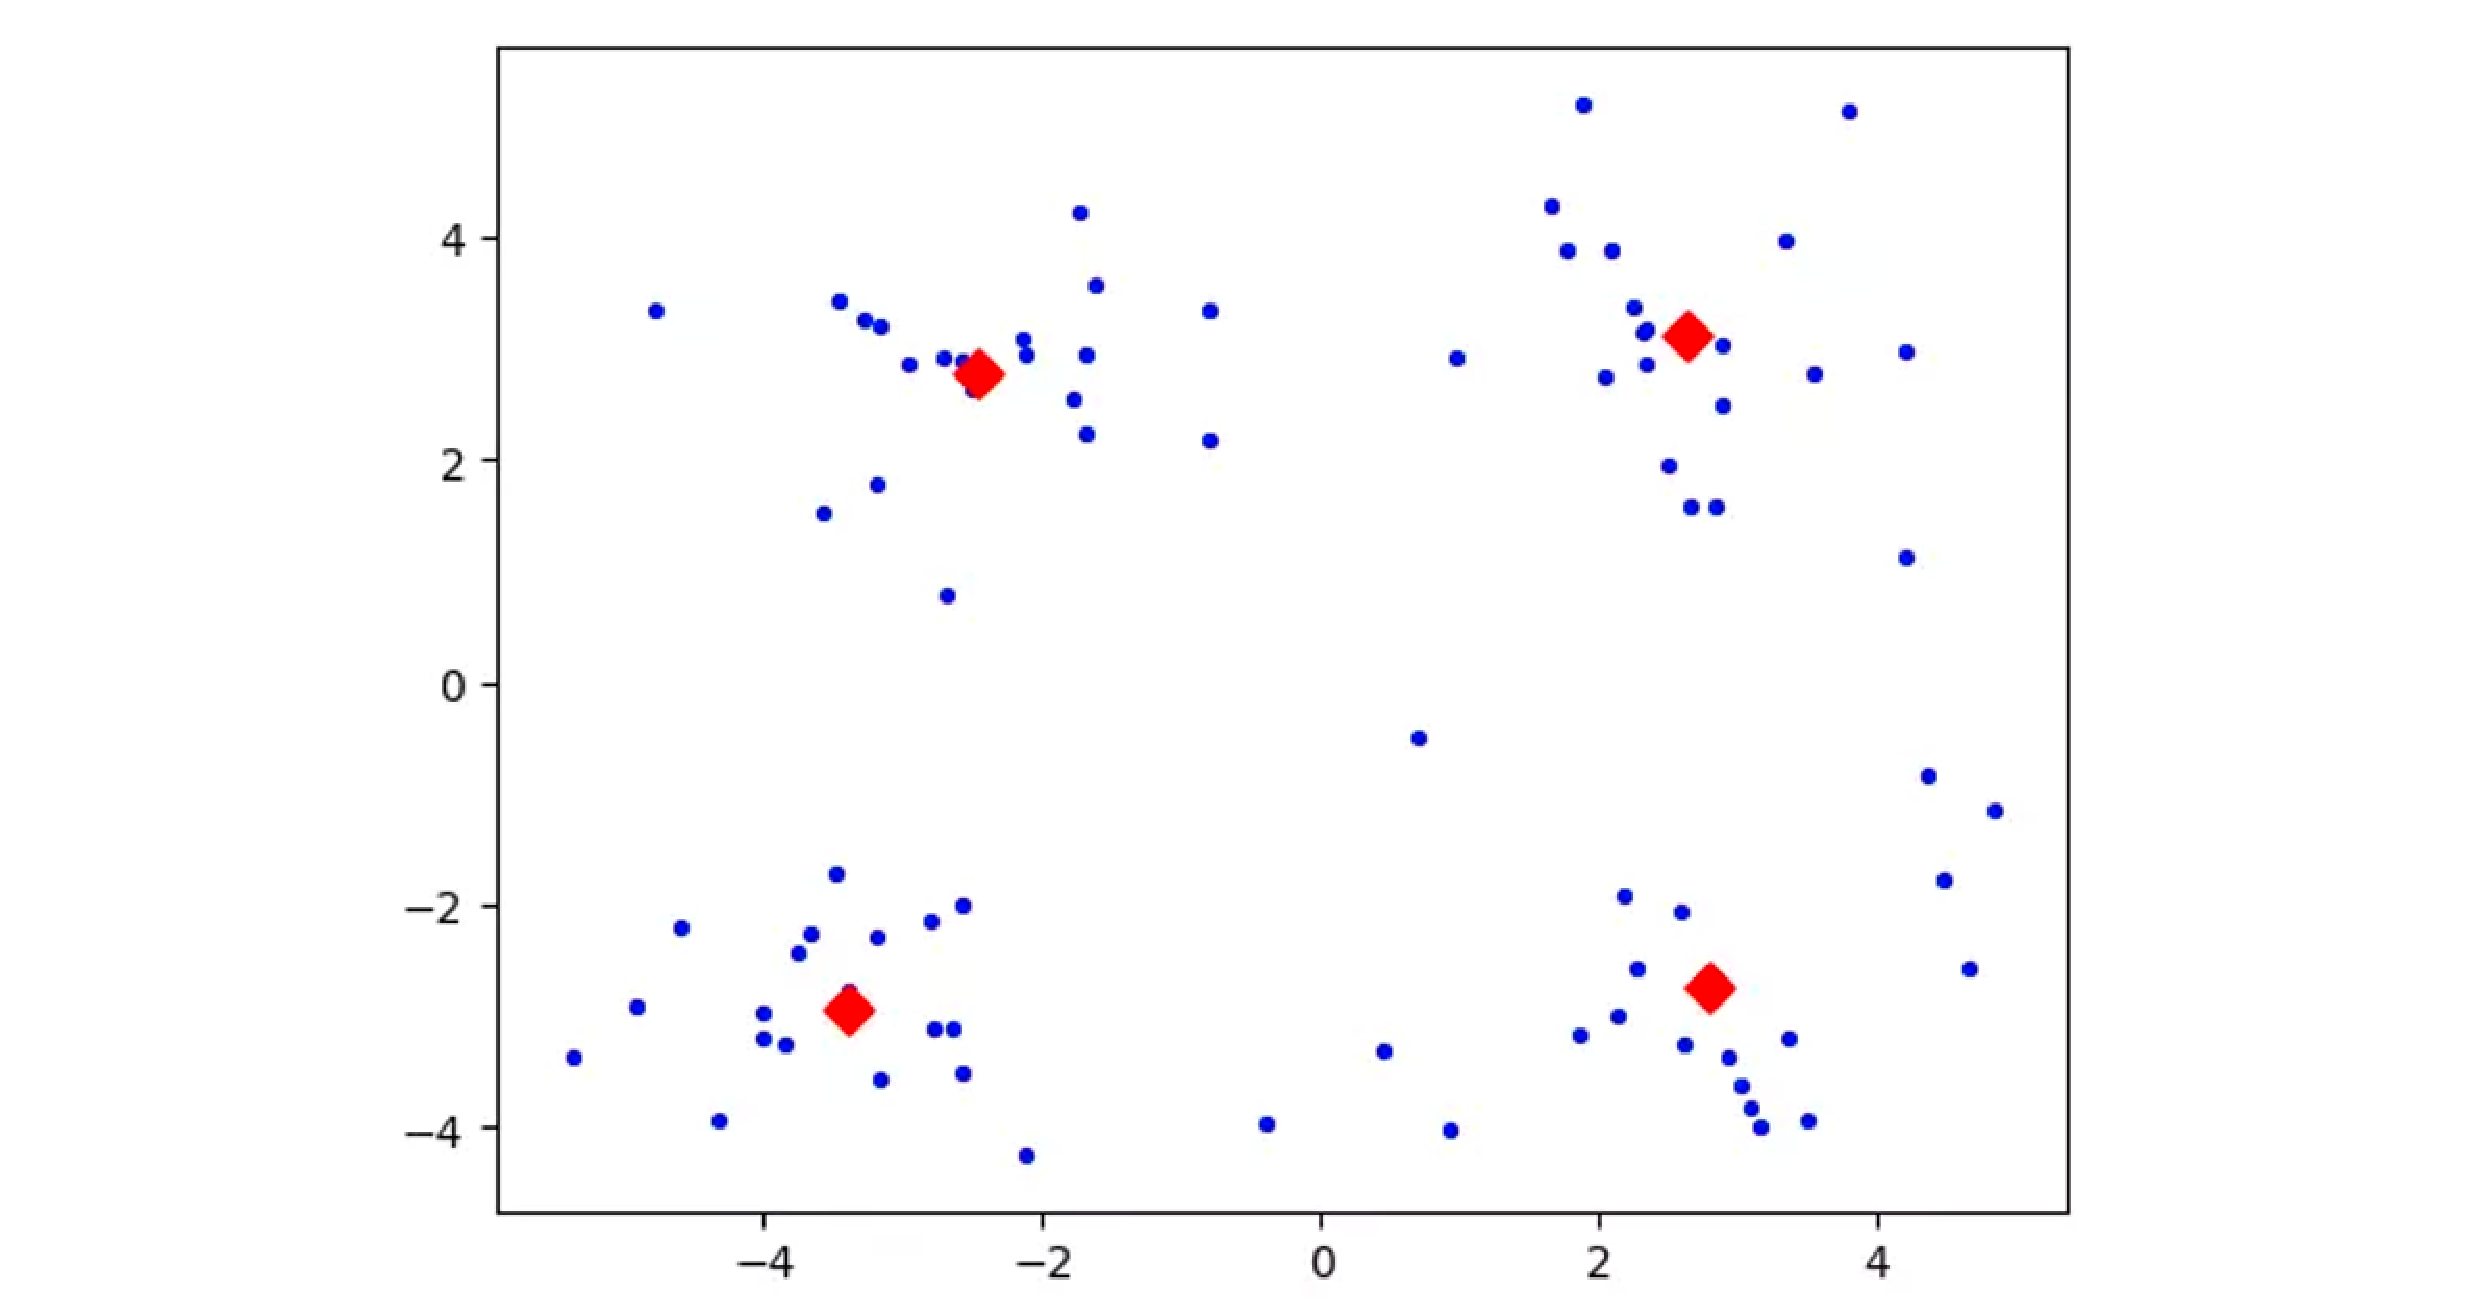
\includegraphics[height=8cm,width=16cm,angle=0,scale=1]{42.eps}
  \caption{聚类分布状态图}\label{42}
     \end{figure}

从上图\ref{42}中的数据分布可以看出,样本点大致分为四簇。所以设置初始聚类中心 $k=4$,如果对数据不是很了解,可以先设置一个$k$,进行聚类之后,再根据结果的聚类效果来调整聚类中心的数量。上图可以看成二维坐标,其中每一个点都有相对应的x坐标和y坐标,通过欧几里得距离公式计算出SSE。Kmeans算法的计算流程如下所示:

(1)首先确定一个$k$值,即我们希望将数据集经过聚类得到$k$个集合。一般而言$k$值并不是事先所知晓的需要尝试多次。

(2)从原数据集合中随机确定$k$个点作为聚类中心。

(3)对数据集中每一个点,计算其与每一个质心的距离(如欧式距离),离哪个质心近,就划分到那个质心所属的集合。

(4)把所有数据归好集合后,一共有$k$个集合。然后重新计算每个集合的质心。

(5)重复步骤3至步骤5,直到集合之间质心间的距离差低于某个阈值算法迭代结束。

通过上述的步骤基本上可以将一组数据划分成为$k$个聚类,本文将其转化为数学表达式,假设簇划分为 $(C_1,C_2,C_3,....,C_N)$, 则本实验的目标是最小化平方误差E:

\begin{equation}\label{emd}
\centering
      E=\sum_{i=1}^n\sum_{x\in C_i}^n||x-u_i||_2^2
               \end{equation}

其中$u_i$为$C_i$的均值向量其表达式为:

\begin{equation}\label{emd}
\centering
     u_i=\frac{1}{\ |C_i|}\sum_{x\in C_i}^{ }x
               \end{equation}

为了进一步理解kmeans算法,本章以二维坐标系为例,讲述如何划分聚类。在二维坐标系中有6个点分别为$p1(0,0),p2(1,2 ),p3(3,1),p4(8,8),p5(9,10),p6(10,7)$,点与点之间的距离直接使用欧几里得距离公式计算,如果点并不是二维的坐标轴上,而是在三维、四维甚至$n$维,其距离计算公式为对应位两两相减求平方和之后开更根号。由于数据量较小,通过观察可得本数据可以划分为两个聚类,为了演示效果直接令$k=2$。初始时随机选两个点$p1$和$p2$,计算出剩余点与其距离如下表\ref{ptabl1}所示:

\begin{table}[H]
\centering
\caption{测试集的划分和各种块出现的频率}\label{ptabl1}
\begin{tabular}{p{4cm}<{\centering}p{4cm}<{\centering}p{4cm}<{\centering}}
\toprule
\textbf{坐标点}&	\textbf{P1}&     \textbf{P2}\\
\midrule
P3	&3.16	&2.24\\
P4	&11.3	&9.22\\
P5	&13.5	&11.3\\
P6	&12.3	&10.3\\
\bottomrule
\end{tabular}
\end{table}


按照距离为原则划分两组中的数据为:组A中只有$p1$,组B中为其他点。
第二步分别计算A组和B组的质心,A组质心为$p1=(0,0)$,B组质心为$pB=(6.2,5.6)$,质心的计算公式为簇中各个向量相加取平均值即可。第三步,以质心为原点计算每一个点到质心的距离再次分组距离分布如下表\ref{ptabl2}所示:

\begin{table}[H]
\centering
\caption{测试集的划分和各种块出现的频率)}\label{ptabl2}
\begin{tabular}{p{4cm}<{\centering}p{4cm}<{\centering}p{4cm}<{\centering}}
\toprule
\textbf{坐标点}&	\textbf{P1}&     \textbf{P2}\\
\midrule
P2	&2.24	&6.3246\\
P3	&3.16	&5.6036\\
P4	&11.3	&3\\
P5	&13.5	&5.2154\\
P6	&12.2	&4.0497\\
\bottomrule
\end{tabular}
\end{table}

第二次分组结果为组$A$:$p1$、$p2$、$p3$。组$B$:$p4$、$p5$、$p6$。再次计算质心轮询上面的步骤直至组A和组B中的点不发生变化,迭代结束。根据上述实验思路给出具体的算法流程伪代码如下所示:

\begin{algorithm}[!h]
	\caption{Kmeans}%算法标题
	\begin{algorithmic}%一行一个标行号
        \STATE 输入$:$   $ $类簇个数K,迭代终止阈值$\phi$,最大迭代次数$MAX\_COUNT$
        \STATE 输出$:$   $ $聚类结果
        \FOR{$k=0$ to $K$}
        \STATE $center_k$ = $rand()\%COUNT$ //初始化K个类簇的聚类中心
        \ENDFOR
        \FOR{$k=0$ to $MAX\_COUNT$}
        \FOR{$t=0$ to $T$}
        \STATE $For$ $every$ $x_i$ //所有数据对象
        \STATE $Dis(x_i,center_k)$ //将$x_i$归于某一个聚簇中
        \ENDFOR
		\FOR{$k=0$ to $K$}
        \STATE $center_k=avg(cluster(k))$ // 将每一个聚簇的平均值作为新的聚类中心
        \ENDFOR
        \STATE $Diff$ = $new(cluster)-old(cluster)$
        \IF{$Diff <=\phi$}
		\STATE $return$  $res$ // 如果新旧聚簇无明显变化则终止循环
		\ENDIF
        \ENDFOR
        \STATE $return$  $res$
	\end{algorithmic}
\end{algorithm}

Kmeans算法其优势是简单且易于实现,收敛速度快,对于结果密集型且区别明显的聚类簇分类效果好,但是其缺陷也非常明显,首先我们需要手动确定聚类数$K$,若原数据集并不能直接分为$k$个聚类有$2k$或者数据集较为分散没有明显特征,kmeans算法效果就会较差。其次kmeans对初始质心的选取依赖较大,不同的随机种子对结果影响非常明显。

因此有学者提出了kmeans++算法,其改进主要针对kmeans算法会随机选取初始质心。kmeans++在质心选取之前还进行了几个步骤,第一步从原数据集合中任意挑选出一个数据作为初始聚类中心。第二步,计算出集合中其他数据与初始聚类中心之间的距离,并将其相加,然后取随机值$r$,若$r$等于某一个数据与聚类中心之间的距离则将当前数据设置为新的聚类中心。第三步,重复上述步骤,直到确定所有的聚类中心。本文所使用的的kmeans++算法在第二步与传统做法有所不同,本人的做法为,若原数据集中有$x$个数据点,求出将$x$个数据点与聚类中心之间的欧式距离,选取其中最远的距离对应的数据作为第二个聚类中心,依次迭代获取最终的初始聚类中心。

\section{聚类算法结合测试集选取基向量}

\subsection{聚类算法的选择}

本人使用了多种聚类算法进行相关实验,包括基于密度的dbscan聚类算法、基于机器学习的马尔科夫模型以及基于均值漂移相关的聚类算法。基于密度聚类的算法过于依赖密度的大小,密度又取决于邻域范围的设定以及邻域中列向量个数的设定。实验结果表明kmeans++ 算法能较好地结合原测试集,提高压缩率。dbscan聚类算法虽然可以自动确定聚类个数,但是需要设置$\epsilon$-邻域以及$MinPts$。 本人经过多次尝试发现对于不同的电路,其$\epsilon$-邻域以及$MinPts$均不相同,无法给出统一的标准,而且这两个值需要不断尝试才能获取较好的压缩增益,如果设置不当与随机选取无异。

Kmeans算法主要的缺陷有两点,第一无法确定数据集需要聚类的数目$K$,第二,只能随机选取初始质心。争对这两个缺陷本文给出了解决方案,首先本文根据电路的行来确定需要聚类的数目$K$,这样做有两点好处,第一对于不同的电路都适用,具有通用性。第二,会保证最终的聚类数不会过多,本实验最终要选择聚类中心充当基向量,若聚类数过多会导致基向量过多,增加硬件开销。针对第二个缺陷,本文结合kmeans++的思想,使用一种极大化质心(基向量)距离的选取方式,保证了初始质心(基向量)之间的距离足够远。通过上述两种解决方案,本实验使用kmeans++算法对已填充的原测试进行聚类。下文将介绍详细过程。

\subsection{基向量的选取}

基向量选取完成后,测试集相对应的主分量集也随之确定。本章主要根据kmeans++聚类算法计算出本文所需要的基向量。

在初始基向量的选取过程中,需要进行测试集预填充,由于本人采取拆分压缩的压缩方法,将原测试集中的无关位填充为0即可。本实验所需要的基向量即为将原测试集聚类之后所产生的聚类中心,下面是选取的具体步骤:为了方便表述,将聚类中心使用基向量来表述。

(1)将原测试集进行预填充,并从中任意挑选出一个列向量作为初基向量,由于是随机选取本实验直接使用第一列作为初始基向量。

(2)依次求出原测试集中其他列向量与,已挑选基向量之间的欧式距离,取距离最大的一列作为第二个选取的基向量。

(3)在原测试集中选取其他列向量作为下一个基向量,将其类比为数学公式为$D_x=\max⁡(D_1,D_2,.....,D_N)$,其中$D_1$表示测试集中第一个列向量与基向量之间的最小距离。同理$D_N$表示测试集中第$N$个列向量与基向量之间的最小距离,这个步骤主要保证基向量之间的距离最大。

(4)重复上述步骤直至确定$k$初始基向量,其中$k$的数量由我们原测试集的数据规模决定。

(5)计算出原测试集中每一列与初始基向量之间的距离。

(6)每个列向量均能计算出$k$个距离,$k$个距离就代表$k$聚类,以距离最小为原则将其划分到相应的聚类中。

(7)确定$k$个聚类之后,将每个聚类中的列向量相加之后求平均值,获取新的聚类中心,即新的基向量。

(8)判断新选取的基向量计算的阈值是否小于等于事先给定的阈值,一旦满足迭代终止条件则,当前获取的基向量为本文所求,如果不满足则返回第二步重复计算。迭代条件可以设定为迭代之后类族的中心点不发生变化或者直接初始化迭代的次数。

\vspace{\baselineskip}
\begin{algorithm}[!h]
	\caption{$PrincipalComponentSetGenerationl$ $(T)$}%算法标题
	\begin{algorithmic}%一行一个标行号
        \STATE 输入$:$   $ $初始$K$个基向量
        \STATE 输出$:$   $ $主分量集
        \STATE $N:$ $Number$ $of$ $vectors$
		\STATE $M:$ $Number$ $of$ $columns$
        \STATE $J[1:N,1 ceiling(log2N)]$ : $Base$ $vector$ $matrix$
        \STATE $T[1:N, 1:M]:$ $Test$ $set$ $set$ $size$
        \STATE $Z=Xor(J)$     //将基向量两两间进行异或得到矩阵$Z$
        \STATE $Z=[Z,-Z]$    //将矩阵Z取反与原来的Z组成新矩阵
		\FOR{$i=1$ to $M$}
        \STATE $d$ = $Hamming(Z,T[1:N, i])$     //计算矩阵$Z$与原测试集中第i列的汉明距离
        \STATE $t$ = $min(d)$         $    $  //求出汉明距离$d$中绝对值最小所对应的索引k
        \STATE $Principal$ = $Z[t]$ //提取主分量
        \STATE $PrincipalComponentSet add(Principal)$
		\ENDFOR
        \STATE $Return PrincipalComponentSet$  //返回主分量集
	\end{algorithmic}
\end{algorithm}

\subsection{主分量集的获取}

得到$K$个基向量后,将其两两之间进行异或,可得到一个列向量数为$2^n-1$的矩阵,然后将这个矩阵取反且与原矩阵拼成一个新的矩阵,计算测试集中的列与新矩阵中的每一列的汉明距离,选取汉明距离最小所对应的列作为主分量,构成主分量集,得到主分量集后,将它与原测试集进行异或,生成残分量集,最后对残分量集进一步压缩。主分量生成的具体过程如算法4.2所示。

例如测试集A的基向量为$\beta_1$(1,0,1,0,1)、$\beta_2$(1,1,0,0,1)、$\beta_4$(0,1,1,1,1)组成,通过基向量两两异或可生成矩阵Z,基向量为三列,对应的Z为7列。

\begin{equation}
Z
=
(\beta_1,\beta_2,\beta_4,\beta_1\bigoplus \beta_2,\beta_1\bigoplus \beta_4,\beta_2\bigoplus \beta_4,\beta_1\bigoplus \beta_2\bigoplus \beta_4)
=
\left[
\begin{array}{ccccccc}
    1&1&0&0&1&1&0\\
    0&1&1&1&1&0&0\\
    1&0&1&1&0&1&0\\
    0&0&1&0&1&1&1\\
    1&1&1&0&0&0&1\\
\end{array}
\right]
\end{equation}


然后将Z取反与原矩阵拼接成为全新矩阵 ,取反即为0和1位置互换。

\begin{equation}
Z
=
\left[
\begin{array}{cccccccccccccc}
    1&1&0&0&1&1&0&0&1&1&1&1&0&0\\
    1&0&1&1&0&1&0&0&0&1&0&1&1&1\\
    1&1&1&0&0&0&1&0&0&1&1&0&0&1\\
    1&0&0&0&0&1&1&0&1&0&0&1&0&1\\
    1&1&0&1&0&0&0&0&0&0&1&1&1&0\\
\end{array}
\right]
\end{equation}

最终计算出测试集A中的每一列与矩阵$Z$每一列的汉明距离$dis$,将$dis$所对应 中的列向量作为当前测试集中相应列的主分量。例如测试集中第二列$β2(1,1,0,0,1)$ 与矩阵$Z$中第二列(1,1,0,0,1)的汉明距离为0,则原测试集第二列的主分量为(1,1,0,0,1)。依此类推,直到计算出原测试集每一列所对应的主分量,构造出主分量集。最终将主分量集合原测试集进行异或,计算出相应残差集,获取压缩率。

\section{实验结果与分析}

本实验中选择的kmeans++算法,需要预先设定聚类中心的个数$k$,聚类数$k$定义得过少或者过多对结果均会产生一定的影响。针对此问题,本文分两个步骤进行了相关实验。第一部分根据电路大小选取基向量个数,并取得压缩率,同时与其他拆分压缩所取得的压缩率进行对比。第二部分,由于基向量需要存储代价,基向量的选取不能无限制的增加,本人在一定范围内动态增加或者减少基向量个数,观察压缩率的变化情况,大致绘制出基向量--压缩率之间的趋势变化图。

\subsection{根据电路大小确定基向量数}

根据电路大小选取基向量,其选取方式为$k=ceil(\log_2^N⁡)$其中$N$为测试集的行数。为了验证聚类算法的有效性,本文对S5378、S9234、S13207、S15850、S38417、S38584等电路进行了实验,下文将对其中部分电路做具体描述,同时与其他压缩方式所得的压缩增益做对比。

实验结果如下表\ref{ptabl3}-\ref{ptabl7}所示,本文选取了FDR、EFDR、ALT-FDR、RL-Huff、VIHC以及Golomb六种编码方式对变换拆分之后的残差集进行压缩,同时与使用哈达码变换、直接预填充方式获取的压缩率进行对比。

第一列为电路名称,第二列为测试集直接压缩之后的结果,第三列是对哈达码变换拆分之后的压缩率,第四列为对测试集预填充所获取的压缩率,第五列是由kmeans++聚类算法结合拆分压缩所的压缩率。

表\ref{ptabl3}是 FDR 编码在各种情况下的压缩率比较,FDR 编码是一种单游程编码方式,其对连续0子串进行编码,遇到1比特位直接使用00进行编码,当0串越长所对应的码字相对于原串越短,压缩率越高。由表中的数据可知,采用本章方法计算的压缩率比对测试集直接编码平均高20\%,比哈达码变换平均高2.4\%,比预填充方法平均高1.72\%。

\begin{table}[H]
\centering
\caption{FDR编码压缩率(\%)}\label{ptabl3}
\begin{tabular}{p{2.2cm}p{2.7cm}<{\centering}p{3.3cm}<{\centering}p{2.7cm}<{\centering}p{2.7cm}<{\centering}}
\toprule
\textbf{电路}&	\textbf{直接编码}& \textbf{哈达码变换}& \textbf{预填充}& \textbf{本方法}\\
\midrule
s5378&	47.98&	67.51&	68.43&	70.76\\
s9234&	43.61&	66.19&	66.39&	69.59\\
s13207&	81.31&	89.65&	91.69&	92.29\\
s15850&	66.21&	80.66&	81.88&	81.75\\
s38417&	43.27&	72.44&	73.04&	75.35\\
s38584&	60.93&	75.99&	75.09&	77.03\\
平均&	57.22&	75.41&	76.08&	77.80\\
\bottomrule
\end{tabular}
\end{table}

表\ref{ptabl4}展示了 EFDR 编码在不同压缩方法下所获取压缩增益,EFDR 编码是一种双游程编码方式,属于对 FDR 编码的一种扩展,既可以对0 游程进行编码,也可以对1进行编码,对测试集中0和1的数目并没有具体的要求,只需要保证跳变数最少即可,如果测试集中0 和1 相继出现,压缩效果就会比较差,由表可知,采用本章描述的方法所获取的压缩率比对测试集直接编码获取的压缩率平均高 12.37\%,比哈达码变换获取的压缩率平均高 2.37\%,比在预填充方法下获取的压缩率平均高 1.58\%。

\begin{table}[H]
\centering
\caption{EFDR编码压缩率(\%)}\label{ptabl4}
\begin{tabular}{p{2.2cm}p{2.7cm}<{\centering}p{3.3cm}<{\centering}p{2.7cm}<{\centering}p{2.7cm}<{\centering}}
\toprule
\textbf{电路}&	\textbf{直接编码}& \textbf{哈达码变换}& \textbf{预填充}& \textbf{本方法}\\
\midrule
s5378&	53.67&	64.50&	65.60&	67.75\\
s9234&	48.66&	62.74&	62.71&	66.14\\
s13207&	82.49&	88.89&	90.95&	91.60\\
s15850&	68.66&	78.67&	78.88&	79.84\\
s38417&	62.02&	71.63&	71.71&	74.06\\
s38584&	64.28&	73.45&	74.69&	74.60\\
平均&	63.30&	73.30&	74.09&	75.67\\
\bottomrule
\end{tabular}
\end{table}

表\ref{ptabl5}-\ref{ptabl6}展示了 ALT-FDR 编码和 RL-Huff 编码在不同压缩方法下所获取压缩增益。由表可知,采用本章所提出的方法,ALT-FDR 编码和RL-Huff 编码所获取的压缩率比对测试集直接编码平均高12.42\%和13.73\%,比哈达码变换获取的压缩率平均高 3.24\% 和4.45\%,比预填充策所达到的平均压缩率分别高 1.7\%和 1.98\%。虽然ALT-FDR 编码和 RL-Huff 编码都是属于双游程编码,需要根据跳变数最少来进行编码,但是较其他压缩方法使用本方法获取的压缩增益依然是最高的。

\begin{table}[H]
\centering
\caption{ALT-FDR编码压缩率(\%)}\label{ptabl5}
\begin{tabular}{p{2.2cm}p{2.7cm}<{\centering}p{3.3cm}<{\centering}p{2.7cm}<{\centering}p{2.7cm}<{\centering}}
\toprule
\textbf{电路}&	\textbf{直接编码}& \textbf{哈达码变换}& \textbf{预填充}& \textbf{本方法}\\
\midrule
s5378&	49.95&	61.62&	63.54&	65.17\\
s9234&	44.96&	58.31&	58.89&	62.72\\
s13207&	80.23&	86.52&	90.16&	90.88\\
s15850&	65.83&	75.76&	76.78&	77.82\\
s38417&	60.55&	68.40&	68.13&	71.23\\
s38584&	61.13&	69.70&	72.09&	71.97\\
平均&	60.58&	70.06&	71.60&	73.30\\
\bottomrule
\end{tabular}
\end{table}

\begin{table}[H]
\centering
\caption{RL-Huff编码压缩率(\%)}\label{ptabl6}
\begin{tabular}{p{2.2cm}p{2.7cm}<{\centering}p{3.3cm}<{\centering}p{2.7cm}<{\centering}p{2.7cm}<{\centering}}
\toprule
\textbf{电路}&	\textbf{直接编码}& \textbf{哈达码变换}& \textbf{预填充}& \textbf{本方法}\\
\midrule
s5378&	52.58&	64.02&	66.73&	68.59\\
s9234&	47.26&	60.33&	63.16&	67.07\\
s13207&	82.49&	88.71&	92.23&	92.82\\
s15850&	67.35&	77.33&	79.47&	80.57\\
s38417&	63.32&	69.66&	71.43&	74.02\\
s38584&	62.40&	71.05&	72.91&	74.74\\
平均&	62.57&	71.85&	74.32&	76.30\\
\bottomrule
\end{tabular}
\end{table}

表\ref{ptabl7}展示了 VIHC 编码在不同压缩方法下所获取压缩增益,VIHC 编码是一种单游程编码方式,采用“1”最少的原则进行拆分。由下表可知,采用本章所提出算法获取的压缩率比对测试集直接编码获取的压缩率平均高 19.25\%,比哈达码变换获取的压缩率平均高2.39\%,比预填充获取的平均压缩率高 2.02\%。

\begin{table}[H]
\centering
\caption{VIHC编码压缩率(\%)}\label{ptabl7}
\begin{tabular}{p{2.2cm}p{2.7cm}<{\centering}p{3.3cm}<{\centering}p{2.7cm}<{\centering}p{2.7cm}<{\centering}}
\toprule
\textbf{电路}&	\textbf{直接编码}& \textbf{哈达码变换}& \textbf{预填充}& \textbf{本方法}\\
\midrule
s5378&	51.75&	69.63&	70.78&	72.81\\
s9234&	47.23&	69.58&	70.12&	73.25\\
s13207&	83.55&	92.20&	93.74&	94.20\\
s15850&	67.97&	82.96&	83.30&	84.28\\
s38417&	53.39&	74.79&	75.74&	77.86\\
s38584&	62.30&	78.11&	79.50&	79.25\\
平均&	61.03&	77.89&	78.86&	80.28\\
\bottomrule
\end{tabular}
\end{table}

从上表中的结果可知,本方法对比于直接编码、哈达码变换、和预填充这三种方法,所获取的平均压缩率是最高的。

为了验证本方法确实有效,本文除了验证ISCAS’89中所包含的电路,还对b15、b17、b20、b21等大电路进行了相关实验。大电路中虽然拥有较多的无关位,但是电路所包含的比特位比较多有些甚至上百万位,上文中提及的电路大部分都是10万位以内。实验结果如下表\ref{ptabl8}-\ref{ptabl9}所示,第一列为电路名称,第二列为当前电路的行数和列数,第三列是直接编码获取的压缩率,第四列为本方法所达到的压缩率。

表\ref{ptabl8}为各个大电路在FDR编码下的压缩率,可以看出大电路中本身就存在较多的无关位,直接压缩也可取得较高的压缩增益,但是使用本方法比直接编码所获取的压缩率平均提高了近6\%

\begin{table}[H]
\centering
\caption{FDR编码压缩率(\%)}\label{ptabl8}
\begin{tabular}{p{2.2cm}<{\centering}p{5cm}<{\centering}p{3cm}<{\centering}p{3cm}<{\centering}}
\toprule
\textbf{电路}&	\textbf{电路规模}& \textbf{直接编码}& \textbf{本方法}\\
\midrule
b15& 1630*483&	83.26&	91.64\\
b17& 2555*1452&	89.93&	94.10\\
b20& 5510*522&	84.15&	90.54\\
b21& 5496*522&	84.13&	90.63\\
b22& 3369*767&	85.10&	89.94\\
平均&	&   85.31&  91.37\\
\bottomrule
\end{tabular}
\end{table}

下表\ref{ptabl9}为各个大电路在EFDR、VIHC、ALT-FDR和RL-Huff编码下的压缩率,由表中数据可得,本章提及的压缩算法确实有利于提高压缩率,即使电路规模相对较大,也能获得较好的压缩增益。

\begin{table}[H]
\centering
\caption{大电路在直接编码和kmeans++算法下压缩率}\label{ptabl9}
\begin{tabular}{p{1cm}p{1cm}<{\centering}p{1.2cm}<{\centering}p{1.2cm}<{\centering}
p{1.2cm}<{\centering}p{1.2cm}<{\centering}p{1.2cm}<{\centering}p{1.2cm}<{\centering}
p{1.2cm}<{\centering}p{1.2cm}<{\centering}}
\toprule
\multicolumn{1}{c}{\textbf{电路}}& \multicolumn{1}{c}{\textbf{电路规模}} &
\multicolumn{4}{c}{\textbf{直接压缩}} & \multicolumn{4}{c}{\textbf{本方法}} \\
\midrule
&  & EFDR&   VIHC&    AFDR&   RL-Huff& 	EFDR&    VIHC&    AFDR&   RL-Huff\\
\hline
b15& 1630*483&	85.99&	86.72&	85.12&	87.01&	91.08&	92.91&	90.61&	92.04\\
b17& 2555*1452&	91.70&	91.88&	91.10&	92.30&	93.81&	94.90&	93.56&	94.46\\
b20& 5510*522&	86.56&	86.44&	85.81&	87.50&	89.92&	91.96&	89.51&	91.07\\
b21& 5496*522&	86.74&	86.45&	86.04&	87.69&	89.98&	92.09&	89.55&	91.16\\
b22& 3369*767&	86.77&	86.90&	86.00&	87.30&	89.35&	90.99&	88.80&	90.20\\
平均&		 &  87.55&	87.68&	86.81&	88.36&	90.83&	92.57&	90.41&	91.79\\
\bottomrule%%l
\end{tabular}
\end{table}

\subsection{动态选取基向量数}

使用kmeans++算法并不能自动确定电路的聚类数,需要事先给定。虽然上文通过电路行数选取基向量获得了较好的压缩增益,并且在同等条件下相比于其他压缩方法也能取得更高的压缩率,但并不能证明按照电路行数来选取聚类数会获得最高的压缩增益。基于此,本人在研究过程中,动态地选取了基向量数,进一步计算出确定基向量数与获取压缩率之间的关系。

通过对S5378、S9234、S13207、S15850、S38417、S38584等电路进行了实验,下表\ref{ptabl10}是当前算法在FDR编码方式下,压缩率的变化情况,第一列为电路名,第二列为原始压缩率,第三列到第七列为选取7到11个聚类数残差集所能达到的压缩率。

\begin{table}[H]
\centering
\caption{FDR编码压缩率(\%)}\label{ptabl10}
\begin{tabular}{p{1.4cm}p{2cm}<{\centering}p{1.8cm}<{\centering}p{1.8cm}<{\centering}p{1.8cm}<{\centering}
p{1.8cm}<{\centering}p{1.8cm}<{\centering}}
\toprule
\textbf{电路名}&	\textbf{直接编码}& \textbf{7列}& \textbf{8列}& \textbf{9列}& \textbf{10列}& \textbf{11列}\\
\midrule
s5378&	47.98&	70.76&	72.96&	73.57&	74.82&	76.3\\
s9234&	43.61&	68.86&	69.54&	69.59&	70.54&	72.25\\
s13207&	81.31&	91.28&	92.29&	92.76&	93.45&	94.23\\
s15850&	66.21&	81.75&	82.67&	82.69&	84.24&	84.88\\
s38417&	43.27&	75.35&	77.54&	76.03&	76.9&	77.36\\
s38584&	60.93&	76.09&	77.03&	78.05&	79.05&	80.15\\
平均&	57.22&	77.35&	78.67&	78.78&	79.83&	80.86\\
\bottomrule
\end{tabular}
\end{table}

根据上表\ref{ptabl10}中的数据大致绘制出如下的折线图\ref{43},从图中可以看出随着基向量数的增加,压缩率整体呈上升趋势,整体来看当基向量数从7 列增加至8列时压缩率提高了1.32\%,之后随基向量增加压缩增益的增加幅度稍微有所降低。

\begin{figure}[H]
  \centering
  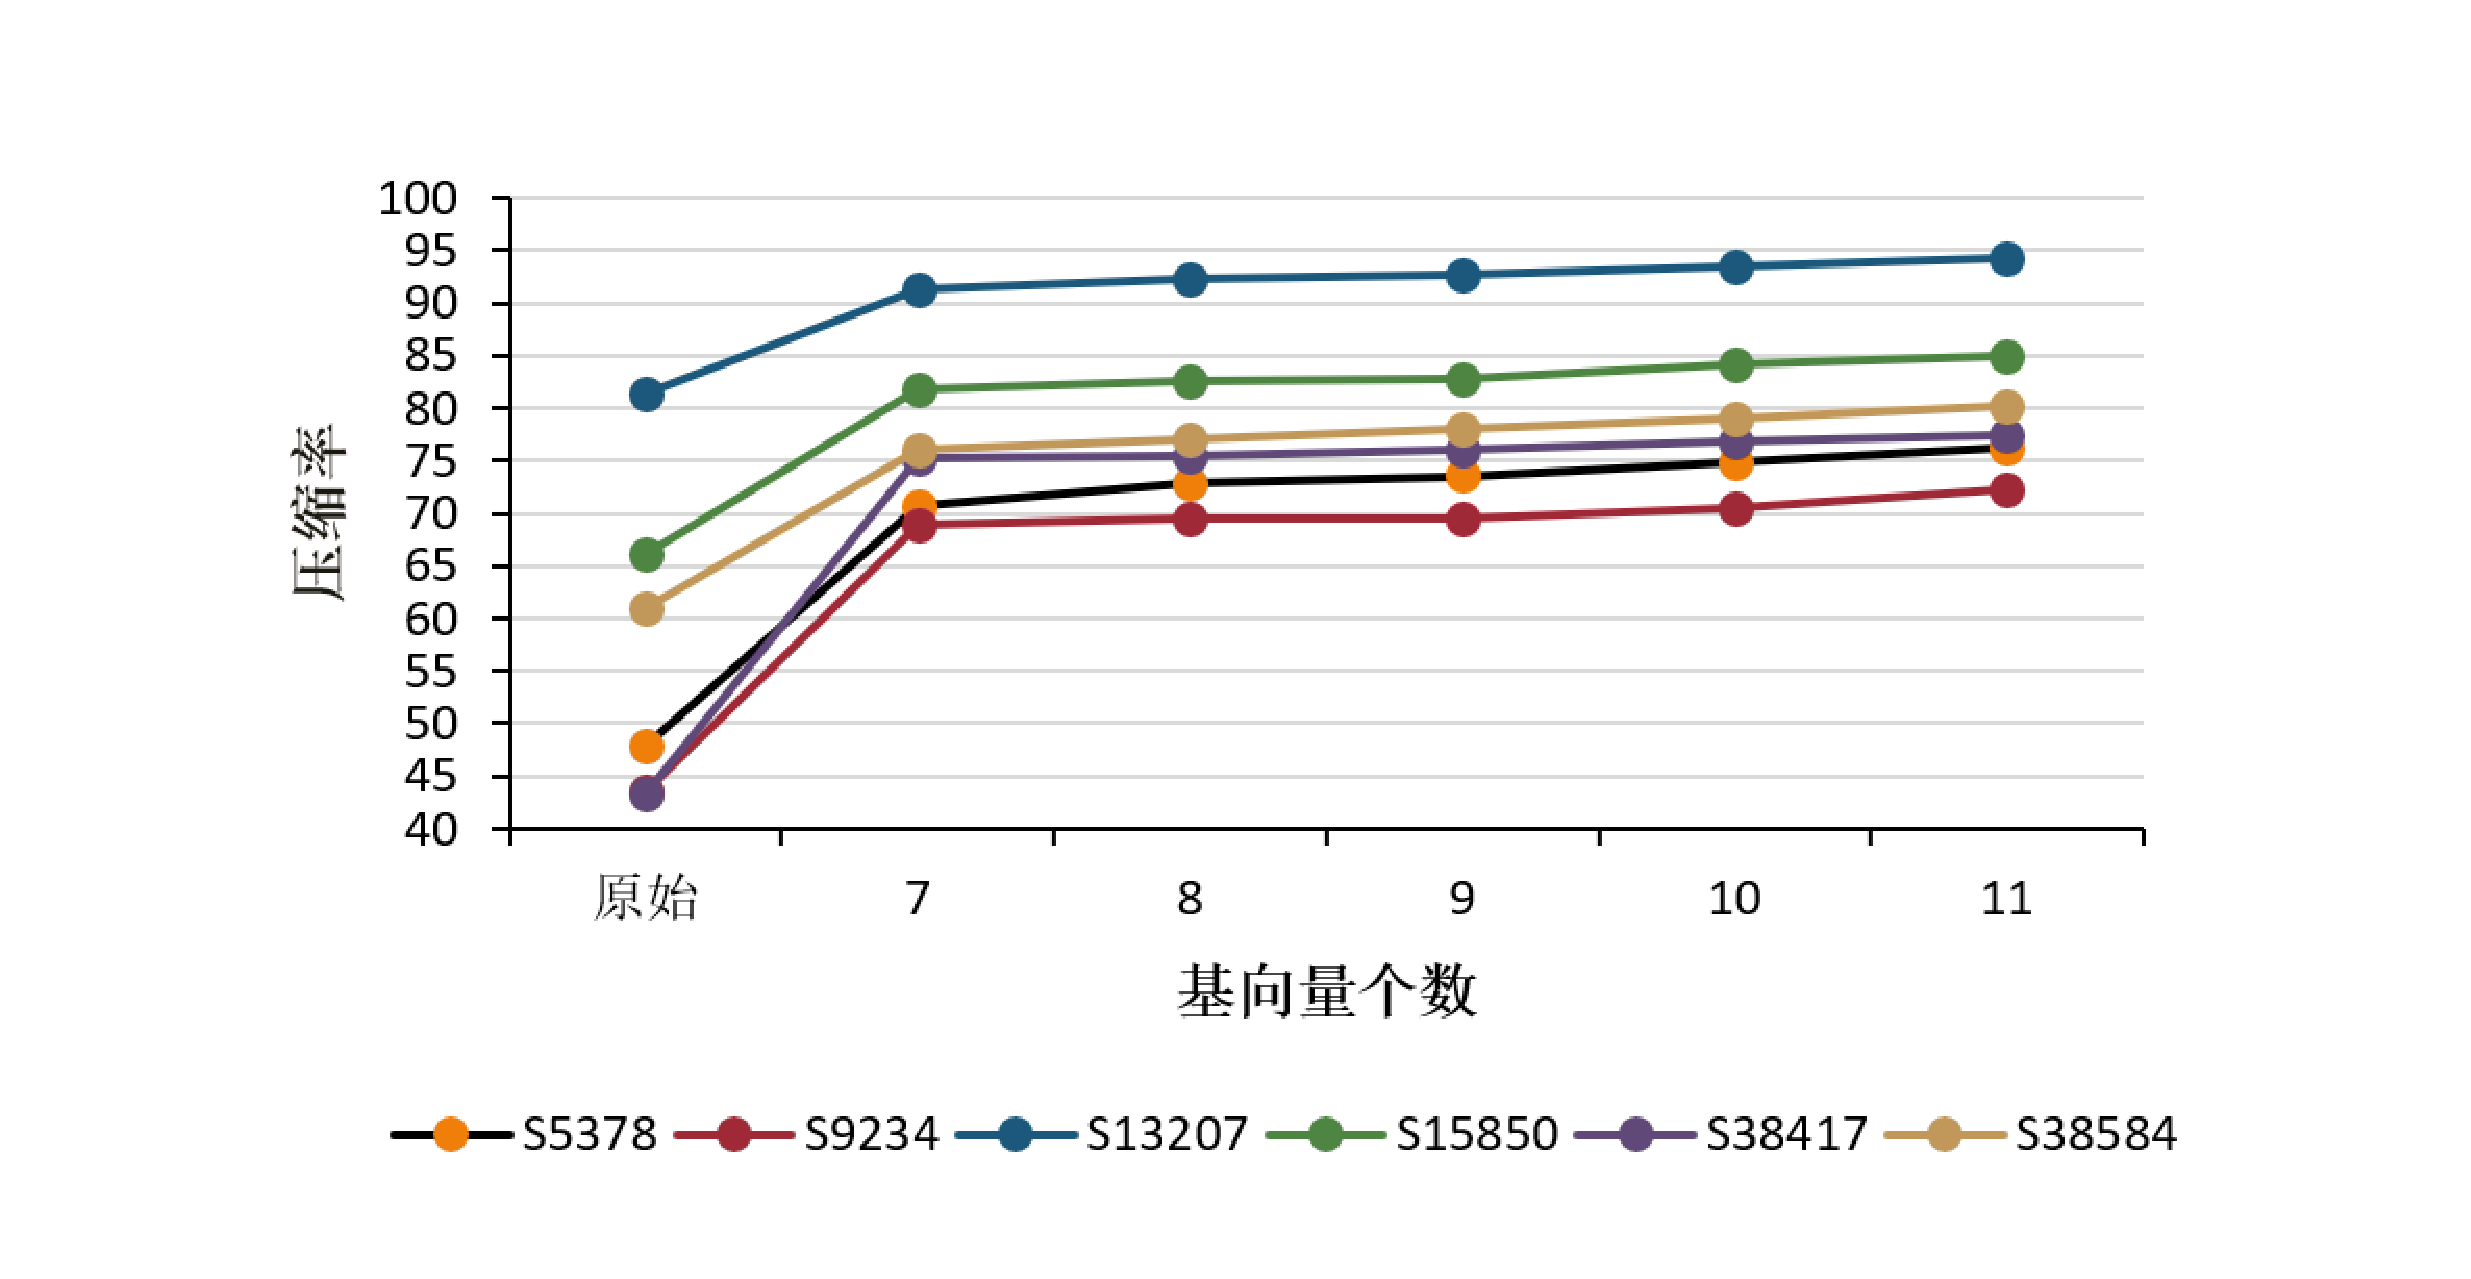
\includegraphics[height=8cm,width=16cm,angle=0,scale=1]{43.eps}
  \caption{FDR编码方式折线图}\label{43}
     \end{figure}

下表\ref{ptabl11}、图\ref{44}是当前算法在VIHC编码方式下,压缩率的变化情况。

\begin{table}[H]
\centering
\caption{VIHC编码压缩率(\%)}\label{ptabl11}
\begin{tabular}{p{1.4cm}p{2cm}<{\centering}p{1.8cm}<{\centering}p{1.8cm}<{\centering}p{1.8cm}<{\centering}
p{1.8cm}<{\centering}p{1.8cm}<{\centering}}
\toprule
\textbf{电路名}&	\textbf{直接编码}& \textbf{7列}& \textbf{8列}& \textbf{9列}& \textbf{10列}& \textbf{11列}\\
\midrule
s5378&	51.75&	72.81&	75.18&	76.02&	77.68&	78.97\\
s9234&	47.23&	72.35&	73.25&	73.4&	74.33&	75.98\\
s13207&	83.55&	93.42&	94.2&	94.55&	95.01&	95.71\\
s15850&	67.97&	84.82&	85.28&	85.42&	86.8&	87.47\\
s38417&	53.39&	77.86&	78.17&	78.64&	79.23&	79.73\\
s38584&	62.30& 	78.42&	79.25&	80.51&	81.62&	82.72\\
平均&	61.03&	79.95&	80.89&	81.42&	82.445&	83.43\\
\bottomrule
\end{tabular}
\end{table}

\begin{figure}[H]
  \centering
  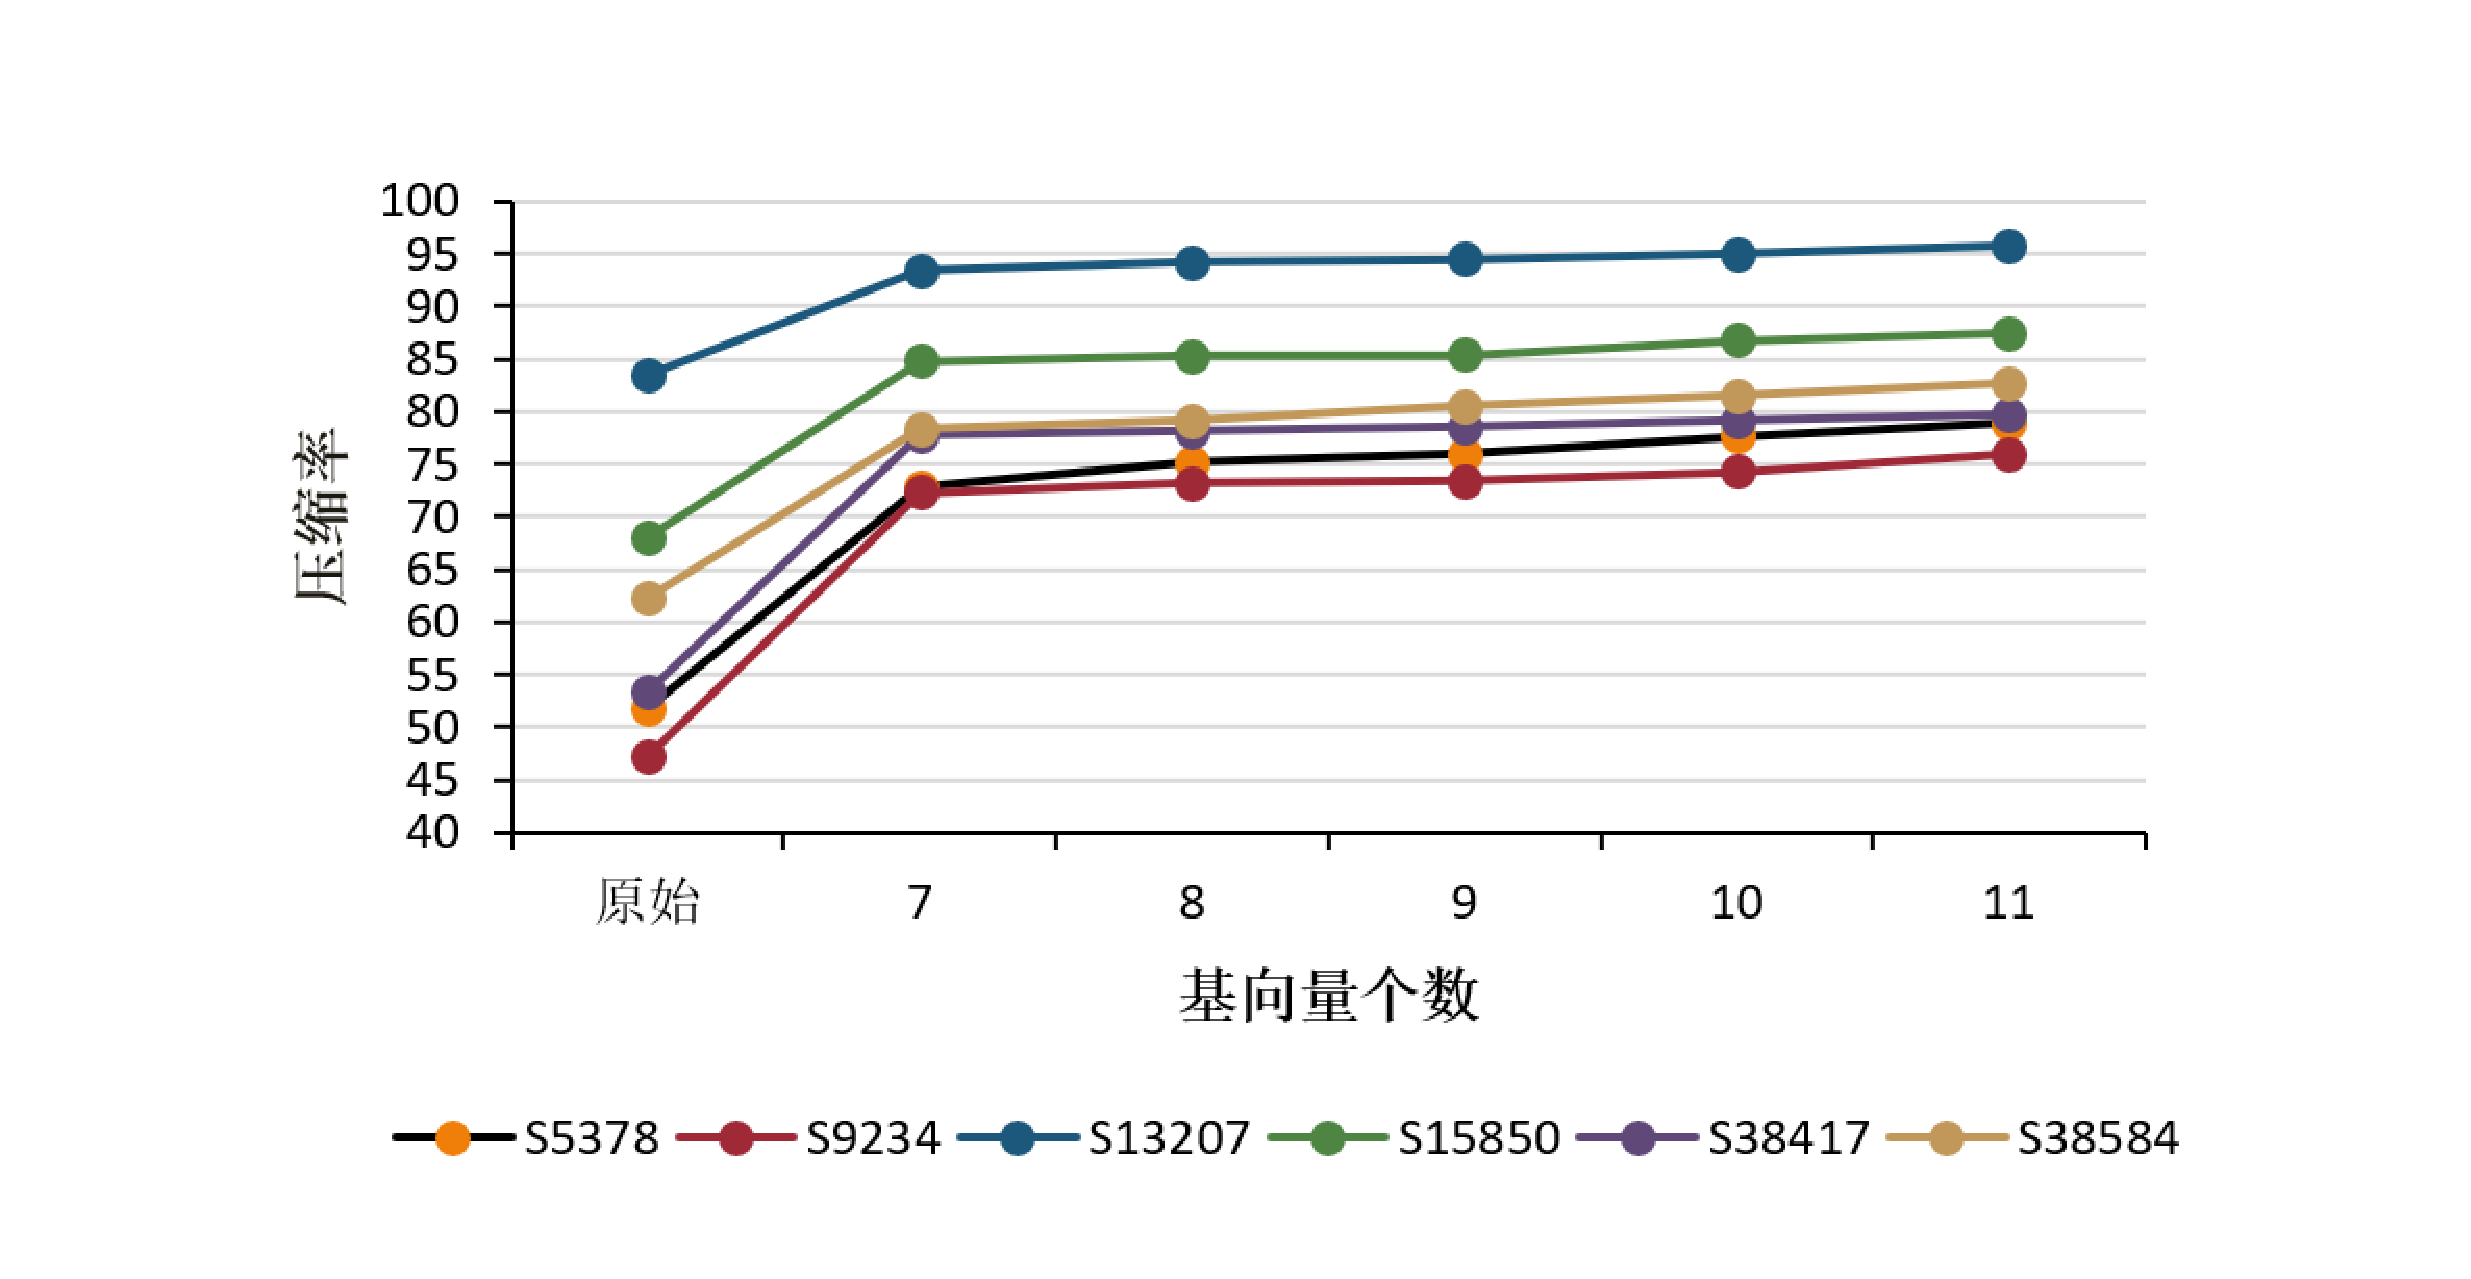
\includegraphics[height=8cm,width=16cm,angle=0,scale=1]{44.eps}
  \caption{VIHC编码方式折线图}\label{44}
     \end{figure}

下表\ref{ptabl12}-\ref{ptabl13}以及图\ref{45}、\ref{46}分别为当前算法在RL\_Huff、AFDR编码下压缩率的变化情况。

\begin{table}[H]
\centering
\caption{RL\_Huff编码压缩率(\%)}\label{ptabl12}
\begin{tabular}{p{1.4cm}p{2cm}<{\centering}p{1.8cm}<{\centering}p{1.8cm}<{\centering}p{1.8cm}<{\centering}
p{1.8cm}<{\centering}p{1.8cm}<{\centering}}
\toprule
\textbf{电路名}&	\textbf{直接编码}& \textbf{7列}& \textbf{8列}& \textbf{9列}& \textbf{10列}& \textbf{11列}\\
\midrule
s5378&	52.58&  68.59&	71.26&	71.79&	73.59&	74.91\\
s9234&	47.26&  66.05&	67.07&	67.05&	68.17&	70.18\\
s13207&	82.94&  91.81&	92.82&	93.23&	93.79&	94.62\\
s15850&	67.35&  80.57&	81.73&	81.77&	83.65&	84.34\\
s38417&	63.32&  74.02&	74.28&	74.71&	75.57&	76.17\\
s38584&	62.40&  73.70&	74.74&	76.13&	77.42&	78.78\\
平均&	62.64&  75.79&	76.98&	77.45&	78.70&	79.83\\
\bottomrule
\end{tabular}
\end{table}

\begin{figure}[H]
  \centering
  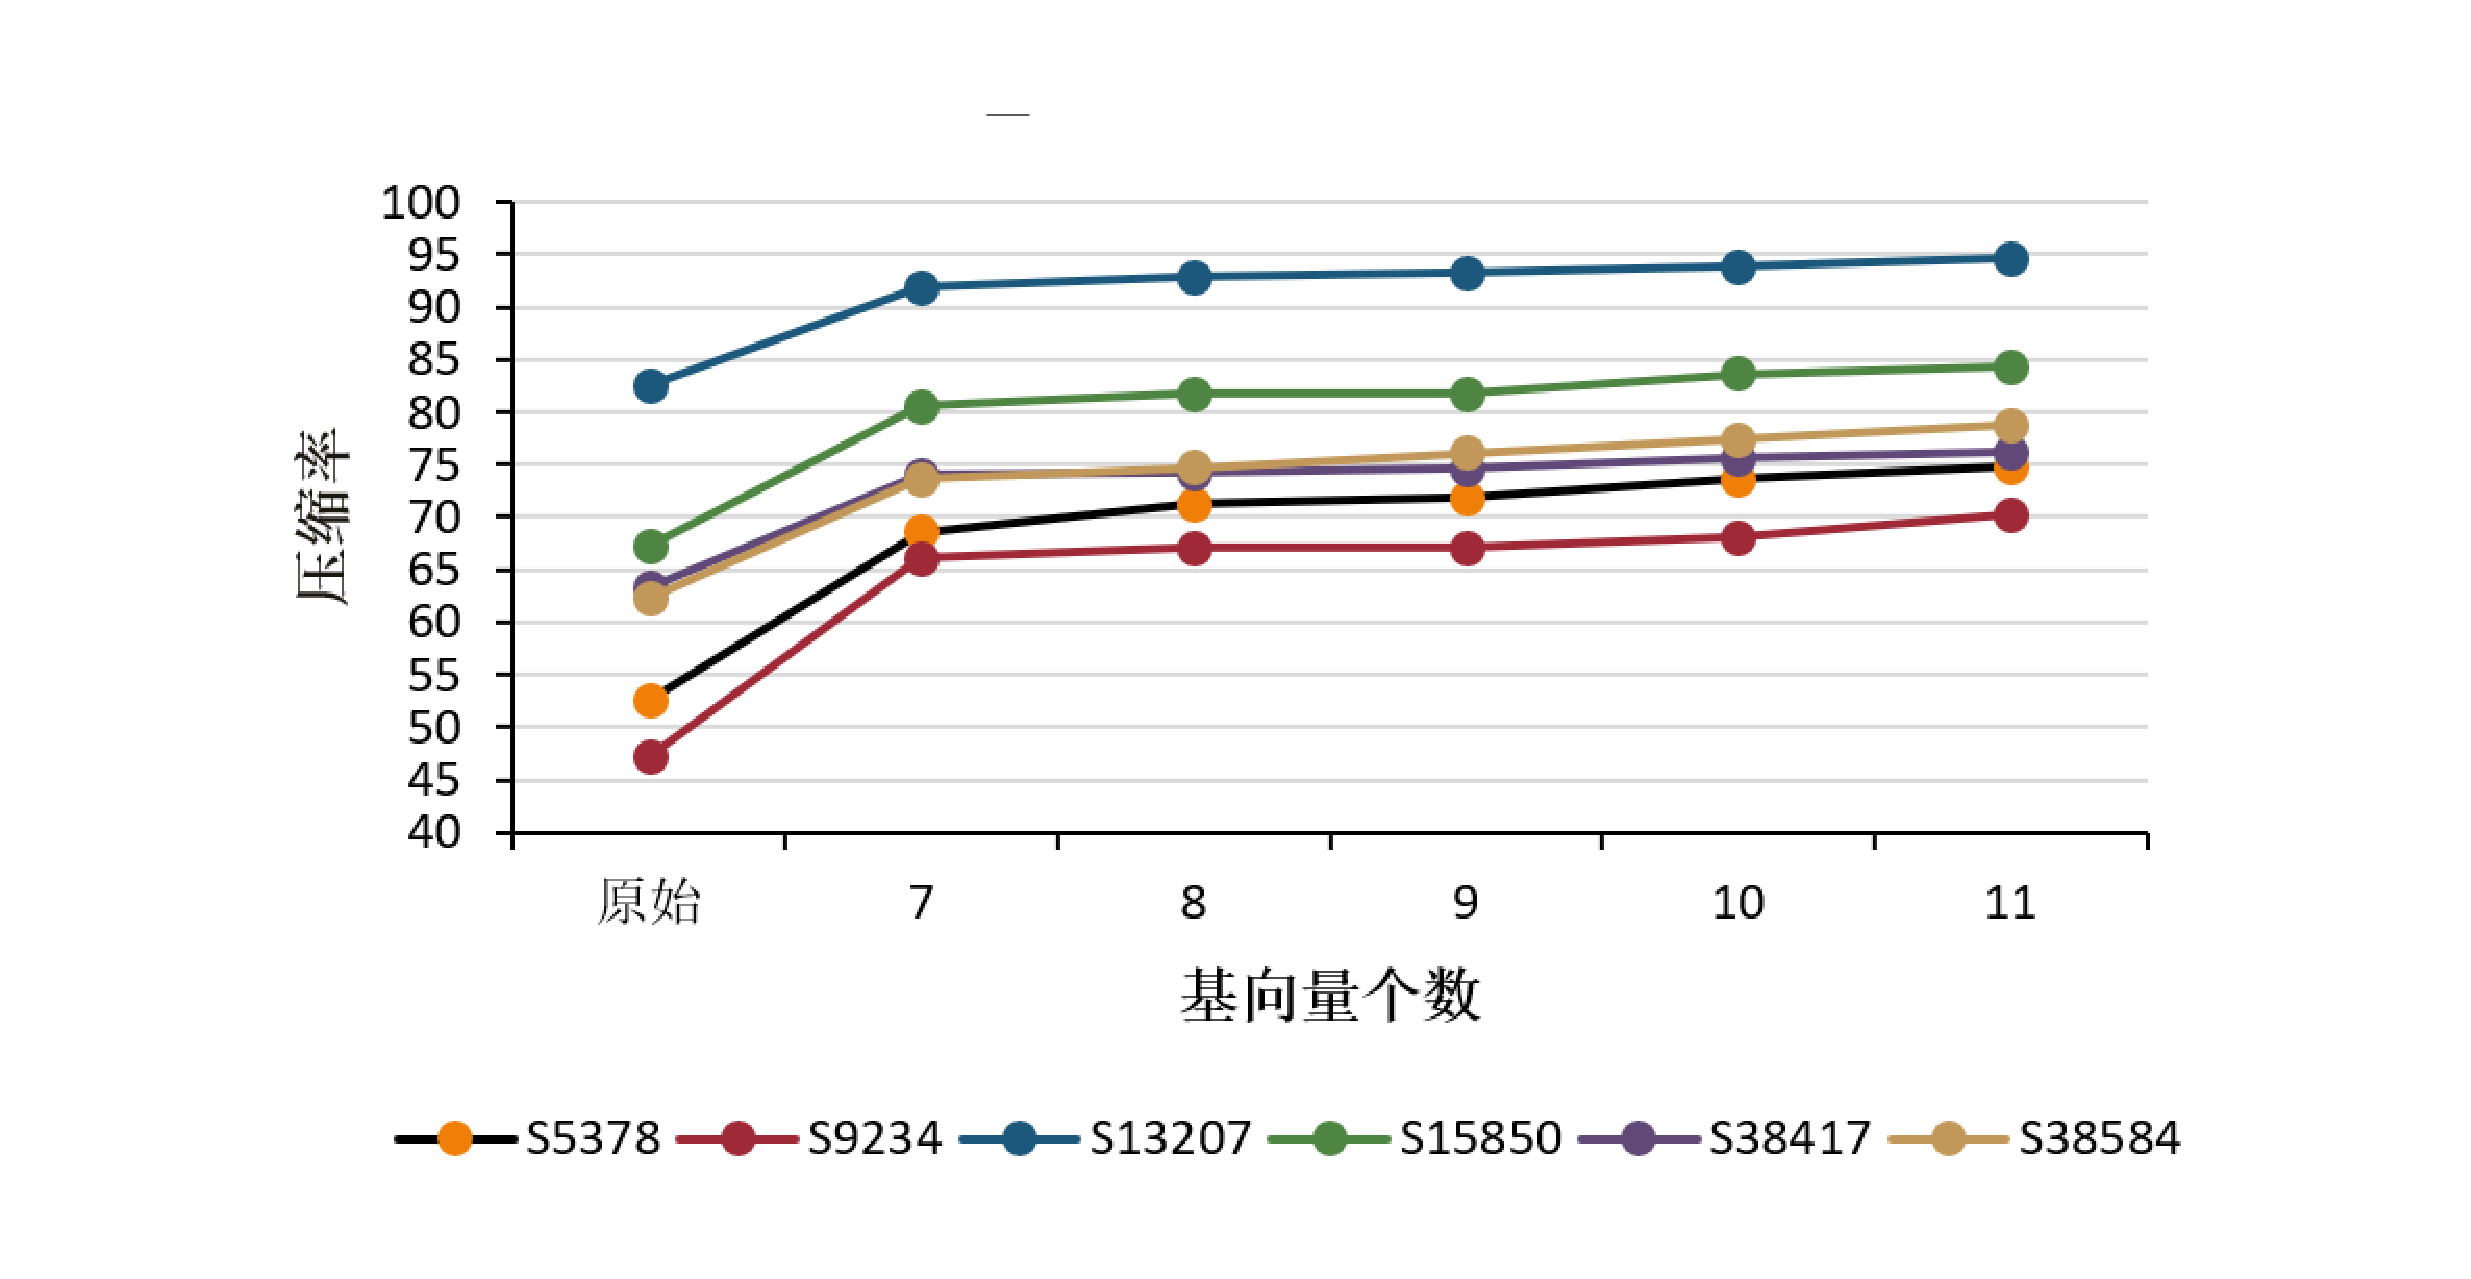
\includegraphics[height=8cm,width=16cm,angle=0,scale=1]{45.eps}
  \caption{RL\_Huff编码方式折线图}\label{45}
     \end{figure}


\begin{table}[H]
\centering
\caption{AFDR编码压缩率(\%)}\label{ptabl13}
\begin{tabular}{p{1.4cm}p{2cm}<{\centering}p{1.8cm}<{\centering}p{1.8cm}<{\centering}p{1.8cm}<{\centering}
p{1.8cm}<{\centering}p{1.8cm}<{\centering}}
\toprule
\textbf{电路名}&	\textbf{直接编码}& \textbf{7列}& \textbf{8列}& \textbf{9列}& \textbf{10列}& \textbf{11列}\\
\midrule
s5378&	49.95&	65.17&	67.66&	68.72&	69.85&	71.53\\
s9234&	45.14&	61.78&	62.72&	63.06&	63.91&	66.11\\
s13207&	80.12&	89.66&	90.88&	91.45&	92.24&	93.18\\
s15850&	65.64&	77.82&	78.96&	78.99&	81.01&	81.66\\
s38417&	60.52&	71.23&	71.38&	71.97&	72.77&	73.34\\
s38584&	61.09&	70.82&	71.97&	73.29&	74.57&	75.93\\
平均&	60.41&	72.75&	73.93&	74.58&	75.73&	76.96\\
\bottomrule
\end{tabular}
\end{table}

\begin{figure}[H]
  \centering
  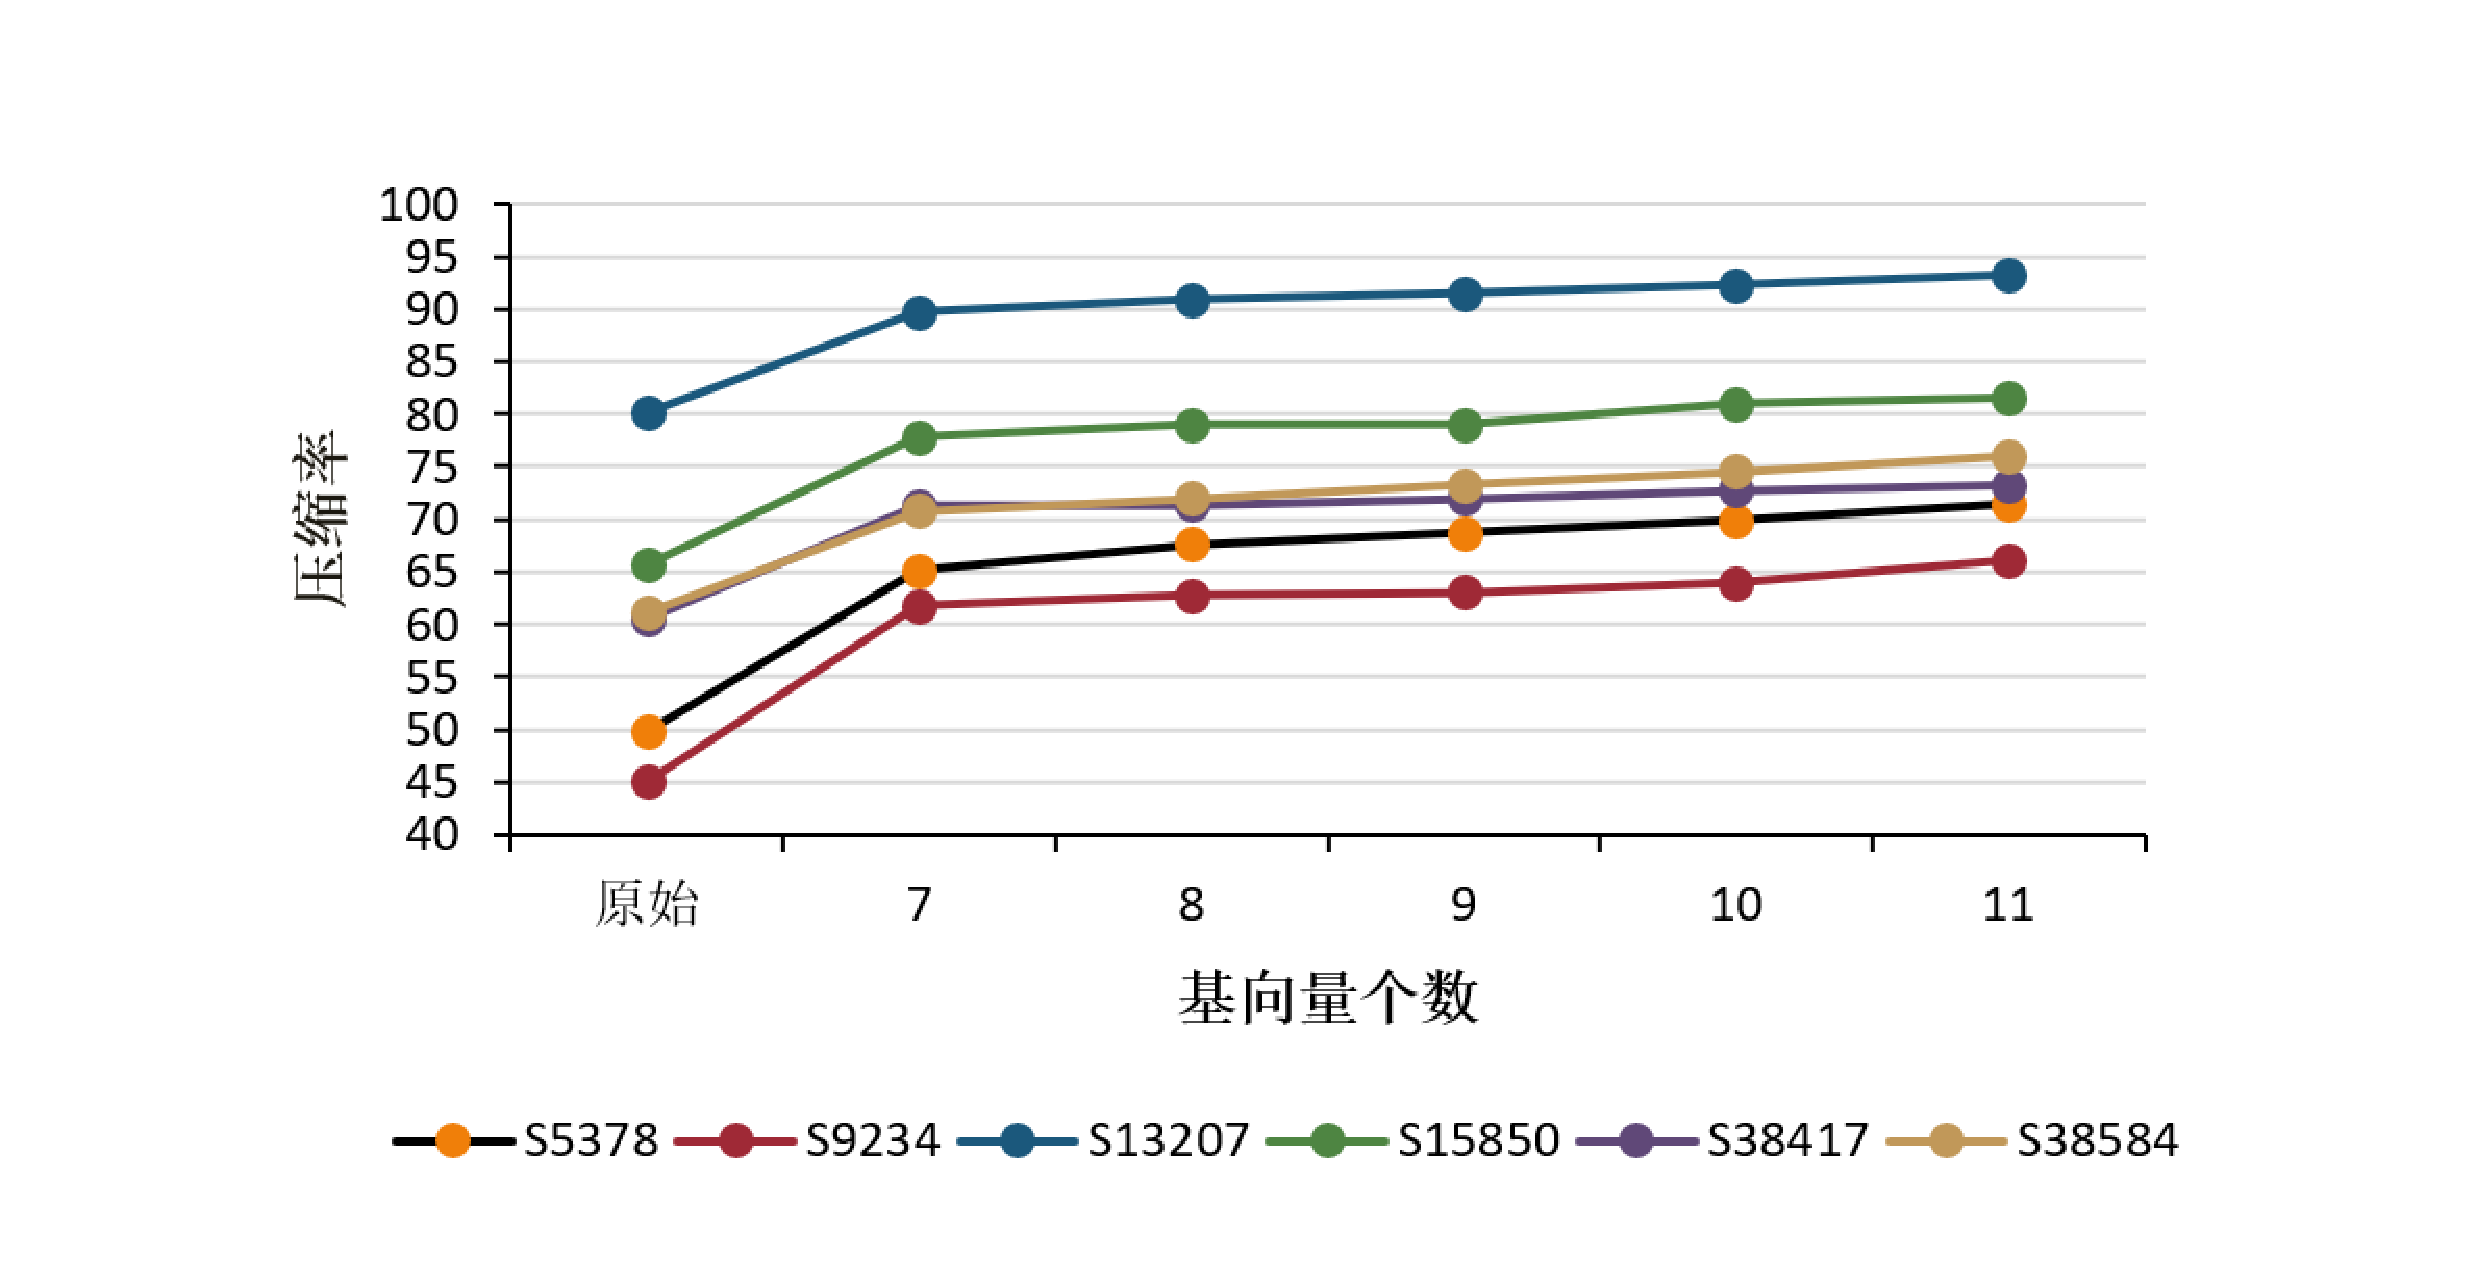
\includegraphics[height=8cm,width=16cm,angle=0,scale=1]{46.eps}
  \caption{AFDR编码方式折线图}\label{46}
     \end{figure}

从上述的折线图可知,随着选取基向量个数的增加,压缩率呈上升趋势,仔细观察可以发现,当基向量增加一个,压缩率提升百分之1左右。总而言之,当前压缩方法无论是根据电路大小确定基向量,还是动态选取基向量均能取得不错的压缩效果。

\section{小结}

本章提出了一种使用聚类算法结合原测试生成主分量的数据压缩方法,该方法先通过预填充方法,去除原测试集中的无关位,然后根据电路大小确定基向量数。由于初始基向量的个数会影响最终的压缩率,并且无法确定初始聚类数,本人进行了动态选取基向量数的相关实验,同时也使用当前压缩方法对大电路测试集进行了压缩。实验结果表明,使用kmeans++聚类算法集合原测试的压缩方法能大大提高压缩率。
